\documentclass{article}
\usepackage[utf8]{inputenc}

\usepackage{graphicx}
\graphicspath{ {./images/} }

\title{Producer Consumer Coarse/Fine Synchronization}
\author{Diaconescu Bogdan Florin}
\date{January 2020}

\begin{document}

\maketitle

\section{Problem statement}
Implement a program to solve the producer-consumer prob-
lem using:\\
a) coarse synchronization\\
b) fine synchronization.\\
The code must be tested with at least 4 producers and the number of consumers
will be given by the number of available virtual CPUs.

\section{Implementation/Solution}
\subsection{Sincronizare grosiera}
Pentru rezolvarea problemei am creat 4 clase:
\begin{itemize}
    \item \textbf{Producer}: clasa ce reprezinta producatorul sub forma unui thread.
    \begin{itemize}
        \item \textit{number} - variabila de tip int prin intermediul careia este identificat producatorul;
        \item \textit{queue} - instanta a clasei \textit{LockBasedQueue} unde sunt puse elementele "produse" de producatori;
        \item \textit{Producer(LockBasedQueue queue, int number)} - constructorul clasei;
        \item \textit{run()}: threadul va executa la nesfarsit urmatoarele instructiuni:
        \begin{itemize}
            \item prin intermediul metodei \textit{put(elementValue,number)} producatorul "number" pune in coada elementul "elementValue";
            \item threadul asteapta 1000 milisecunde.
        \end{itemize}
    \end{itemize}
    \item \textbf{Consumer}: clasa ce reprezinta consumatorul sub forma unui thread.
    \begin{itemize}
        \item \textit{number} - variabila de tip int prin intermediul careia este identificat consumatorul;
        \item \textit{queue} - instanta a clasei \textit{LockBasedQueue} de unde sunt extrase elementele "consumate" de consumatori;
        \item \textit{Consumer(LockBasedQueue queue, int number)} - constructorul clasei;
        \item \textit{run()}: threadul va executa la nesfarsit urmatoarele instructiuni:
        \begin{itemize}
            \item prin intermediul metodei \textit{take()} este extras un element din coada \textit{queue};
            \item este afisat elementul;
            \item threadul asteapta 1000 milisecunde.
        \end{itemize}
    \end{itemize}
    \item \textbf{LockBasedQueue}: clasa ce reprezinta coada in care sunt puse si extrase elementele
    \begin{itemize}
        \item \textit{head} - variabila de tip int ce reprezinta capul cozii;
        \item \textit{tail} - variabila de tip int ce reprezinta coada cozii;
        \item \textit{elementsList} - vector de tipul int in care sunt stocate elementele;
        \item \textit{queueLock} - zavor folosit pentru accesul la coada;
        \item \textit{notFull} si \textit{notEmpty} - cele 2 conditii folosite pentru zavor;
        \item \textit{LockBasedQueue(int maximumLength)} - constructorul clasei;
        \item \textit{take()} - metoda folosita pentru extragerea unui element din coada. Se realizeaza urmatoarele instructiuni:
        \begin{itemize}
            \item se blocheaza zavorul cozii \textit{queueLock.lock()};
            \item cat timp coada este goala se asteapta punerea unui element in coada prin apelarea metodei \textit{await()} pentru conditia \textit{notEmpty}. Aceasta metoda face ca threadul respectiv sa astepte pana cand este notificat de un alt thread;
            \item se extrage un element din coada, deci coada nu mai este plina si se apeleaza metoda signal() care trezeste un thread ce asteapta;
            \item se deblocheaza zavorul si se returneaza elementul extras.
        \end{itemize}
        \item \textit{put(int elementValue, int producerNumber)} metoda folosita pentru a insera elemente in coada. Se realizeaza urmatoarele instructiuni:
        \begin{itemize}
            \item se blocheaza zavorul cozii \textit{queueLock.lock()};
            \item cat timp coada este plina se asteapta extragerea unui element din coada prin apelarea metodei \textit{await()} pentru conditia \textit{notFull}. Aceasta metoda face ca threadul respectiv sa astepte pana cand este notificat de un alt thread;
            \item se adauga un element in coada, deci coada nu mai este goala si se apeleaza metoda signal() care trezeste un thread ce asteapta;
            \item se deblocheaza zavorul cozii.
        \end{itemize}
    \end{itemize}
    \item \textbf{MainClass}: clasa ce contine functia main unde este creata coada, sunt creati producatorii si consumatorii si se incepe executia threadurilor.
\end{itemize}
\subsection{Sincronizarea fina}
Pentru rezolvarea problemei cu ajutorul sincronizarii fine am creat 4 clase:
\begin{itemize}
    \item \textbf{SharedQueue}: clasa ce reprezinta coada in care se vor pune elementele si de unde vor fi extrase.
    \begin{itemize}
        \item \textit{maximumLength} - dimensiunea cozii;
        \item \textit{elementsList} - lista in care se pun si din care se extrag elementele;
        \item \textit{cellLock} - un vector de zavoare pentru accesul la fiecare celula a listei;
        \item \textit{queueLock} - zavor pentru accesul la coada;
        \item \textit{notFull} si \textit{notEmpty} - cele 2 conditii pentru cazul in care coada este plina sau goala;
        \item \textit{SharedQueue()} - constructorul clase;
        \item \textit{put(int value)} - functie ce adauga elementul \textit{value} in coada. Mai intai se blocheaza zavorul pentru celula. Daca lista nu exte plina (\textit{elementsList.size() != maximumLength}) se adauga elementul, iar daca lista este plina (\textit{elementsList.size() == maximumLength}) se asteapta pana cand se elibereaza un loc (\textit{notFull.await()}) apoi se insereaza elementul si se elibereaza zavorul pentru celula.
        \item \textit{take()} - functie folosita pentru extragerea unui element din coada. Mai intai se blocheaza zavorul pentru celula, apoi se verifica daca lista are elemente in ea. In caz afirmativ se extrage elementul, iar in cazul in care nu exista niciun element in lista se asteapta pana se gaseste unul. La final, se elibereaza zavorul pentru celula. 
    \item \textbf{Producer}: clasa ce reprezinta producatorul si implementeaza interfata Runnable.
    \begin{itemize}
        \item Fiecare producator este identificat prin variabila \textit{number};
        \item In functia \textit{run()} se insereaza un element in coada cu ajutorul functiei \textit{put(elementValue)} iar apoi se asteapta 1000 de milisecunde.
    \end{itemize}
    \item \textbf{Consumer}: clasa ce reprezinta consumatorul si implementeaza interfata Runnable.
    \begin{itemize}
        \item Fiecare consumator este identificat prin variabila \textit{number};
        \item In functia \textit{run()} se extrage un element din coada cu ajutorul functiei \textit{take()} iar apoi se asteapta 1000 de milisecunde.
    \end{itemize}   
    \item \textbf{ProducerExecutor}: clasa executor in care se incepe executia producatorului.
    \item \textbf{ConsumerExecutor}: clasa executor in care se incepe executia consumatorului.
    \item \textbf{MainClass}: clasa ce contine functia main de unde se incepe executia programului. Exista un numar de 4 producatori, iar numarul consumatorilor reprezinta numarul procesoarelor virtuale disponibile.
    \end{itemize}
\end{itemize}
\section{Experimental data}

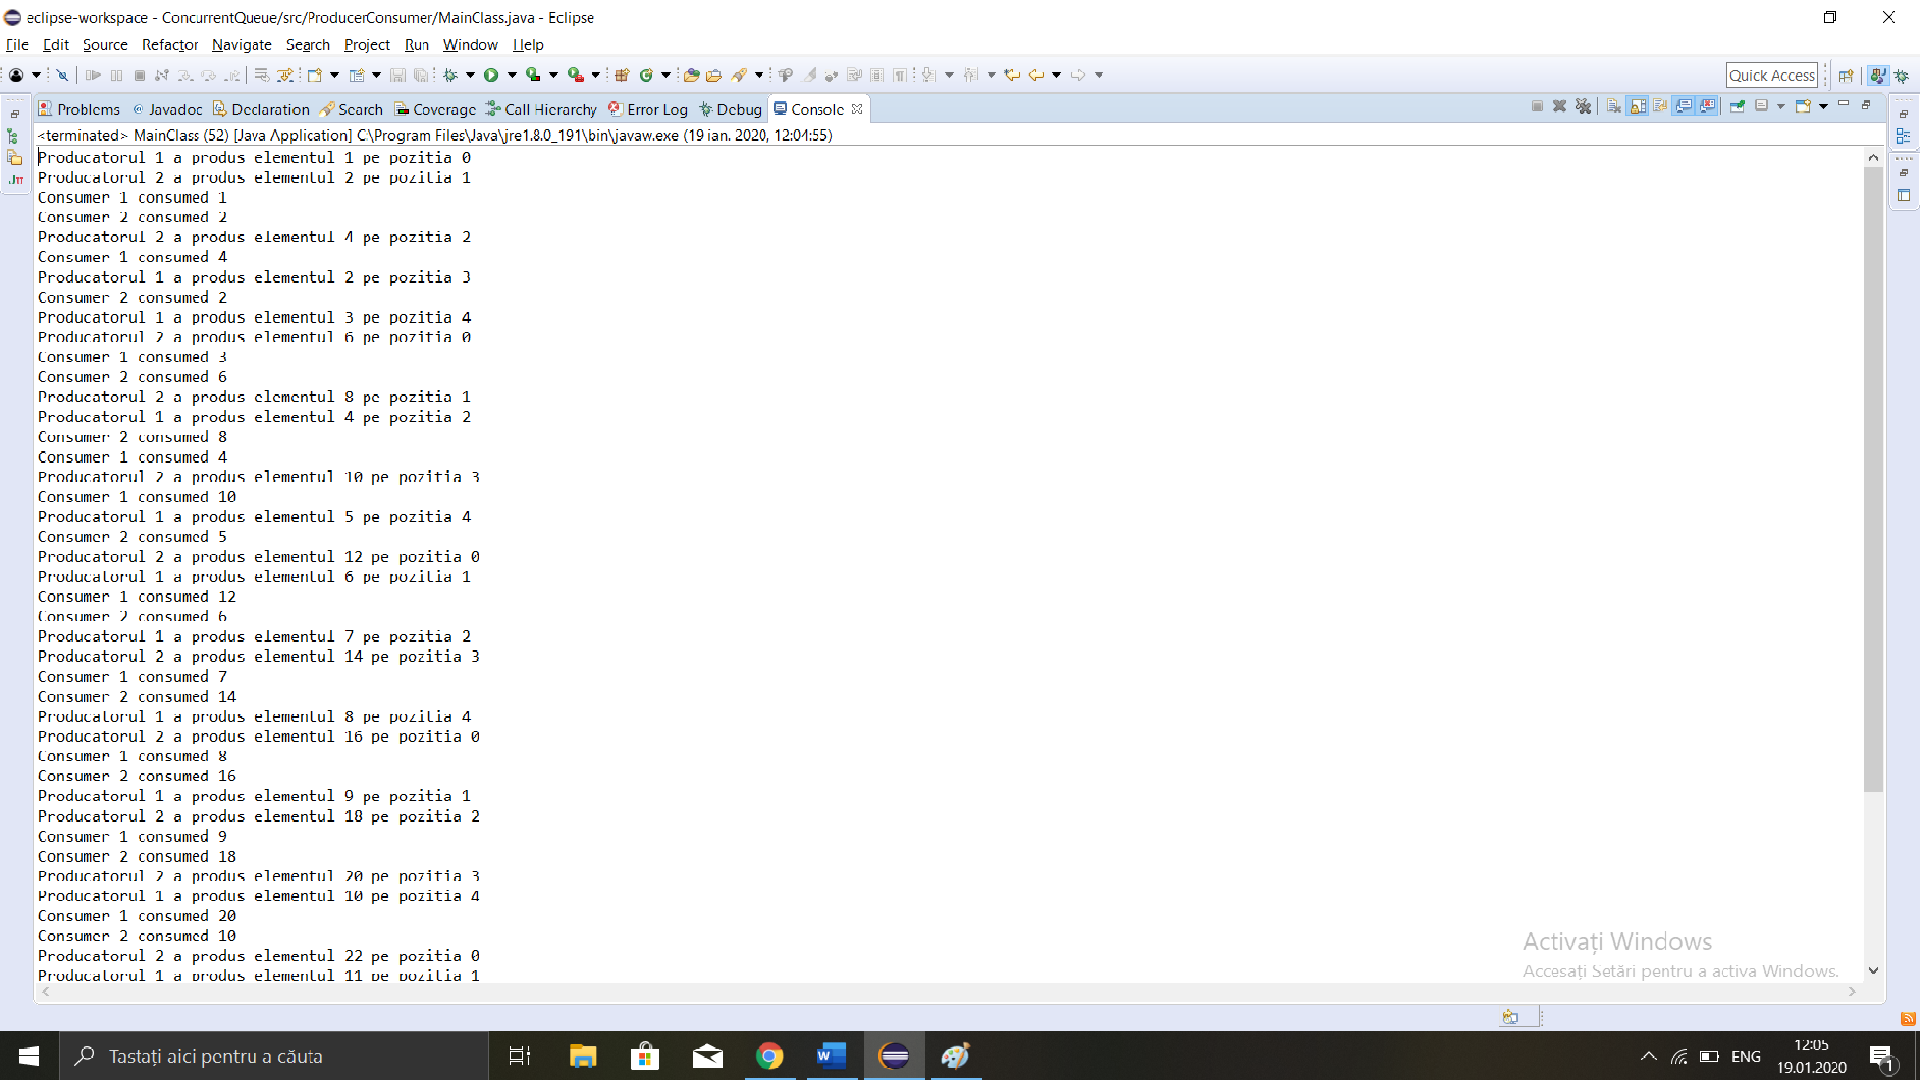
\includegraphics[]{Producer-Consumer.png}

\section{Results \& Conclusions}
Am rezolvat problema "producer-consumer" utilizand sincronizarea grosiera cat si cea fina. Pentru sincronizarea fina a trebuit sa folosesc zavoare pentru accesul la fiecare element din coada, precum si un executor pentru producator, respectiv consumator.\\ 
In ambele metode am creat o coada in care sunt puse si din care sunt extrase elementele. In cazul sincronizarii grosiere, atat numarul producatorilor cat si cel al consumatorilor a fost 2. La sincronizarea fina, au existat 4 producatori, iar numarul consumatorilor a fost dat de numarul de procese virtuale disponibile.
\end{document}
